\documentclass[../Main.tex]{subfiles}
\begin{document}
\section{Ingeniería}
    
    \subsection{Metodología de desarrollo}
    \begin{justify}
    La metodología de desarrollo de software aplicada fue Kanban, después de identificar el tipo de proyecto se determinó que era la metodología que más se ajustaba. En la sección 2.2.5 se explica la metodología Kanban con todos los beneficios que ofrece.
    
    En la implementación se utilizó la plataforma Jira que permite visualizar el flujo de trabajo, establecer los límites de trabajo en curso y la medición del tiempo para cada tarea.
    \end{justify}
    
    \begin{figure}[H]
	\begin{Center}
		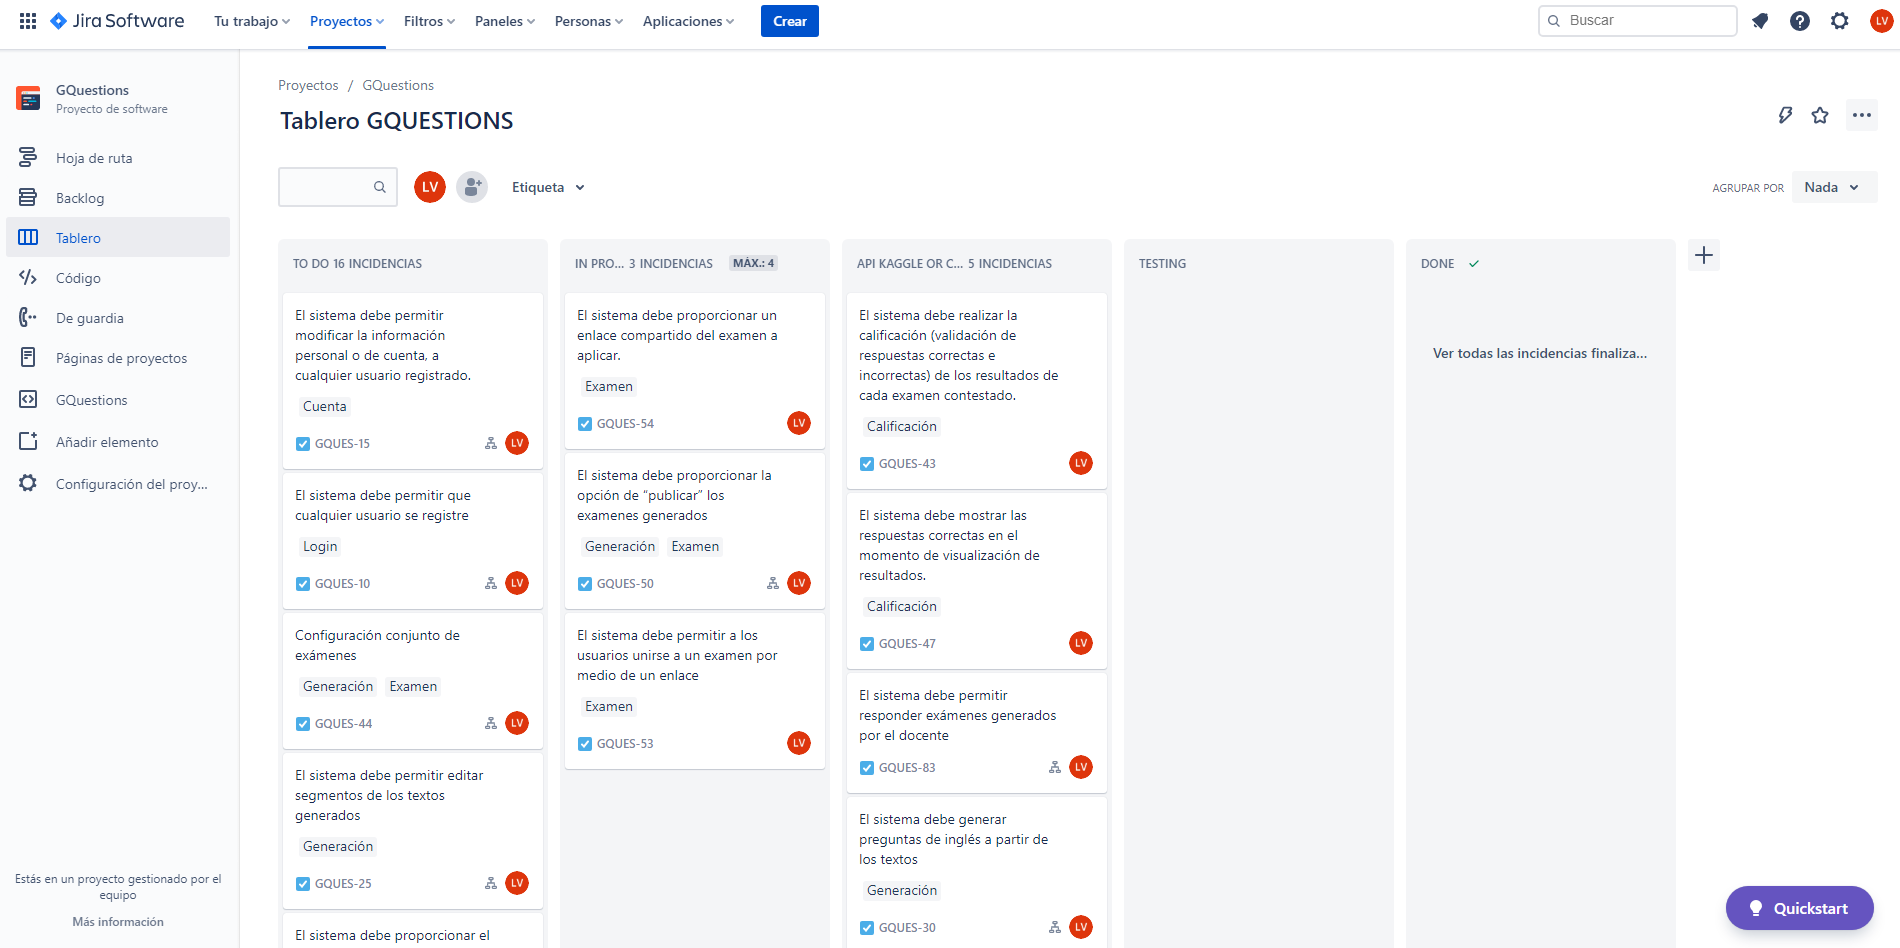
\includegraphics[width=6.4in,height=3in]{Images/TableroJira.png}
	    \caption{Tablero Kanban Jira - GQuestions}
	    Fuente: Elaboración propia
        \label{fig:section}
	\end{Center}
    \end{figure}
    
    
    \subsection{Análisis}
    \begin{justify}
    En esta fase se llevó a cabo el análisis de las necesidades identificadas de acuerdo al problema planteado y las soluciones a brindar por medio de un prototipo web, teniendo en cuenta los objetivos trazados y resultados esperados.
    \end{justify}
    
    \subsubsection{Historias de usuario}
    \begin{justify}
    Con el fin de identificar las funciones del prototipo web que daban valor al cliente se elaboraron las historias de usuario, incluyendo la planeación de tareas a llevar a cabo.
    Se utilizó un formato que permitiera establecer una prioridad a cada historia de usuario de acuerdo a la importancia en el desarrollo.
    
    Este formato contiene la siguiente información: autor, responsable, módulo al que pertenece, prioridad, descripción, validación y finalmente la fecha de creación.
    \end{justify}
    
    \subfile{./TablaHU}
        
    \begin{justify}
    Las demás especificaciones de historias de usuario se encuentran en los anexos.
    \end{justify}
    
    \newpage
    \subsection{Diseño}
    \begin{justify}
    En esta sección se presentan diferentes artefactos de software que son fundamentales para la construcción del producto, conformando la base y el plan de solución del prototipo web.
    \end{justify}
    \subsubsection{Diagrama casos de uso}
    \begin{justify}
    Los diagramas de caso de uso son una descripción de los requerimientos funcionales de un sistema, en él se tienen en cuenta los actores, los escenarios y otros sistemas externos.
    Se empieza con un evento desde un actor hacia el sistema, es importante tener en cuenta que los casos de uso describen que hace un sistema, pero no cómo.
    
    Para tener claro el comportamiento del prototipo web se realizó el diagrama de casos de uso presentado en la siguiente figura.
    
    \end{justify}
        \begin{figure}[H]
	\begin{Center}
		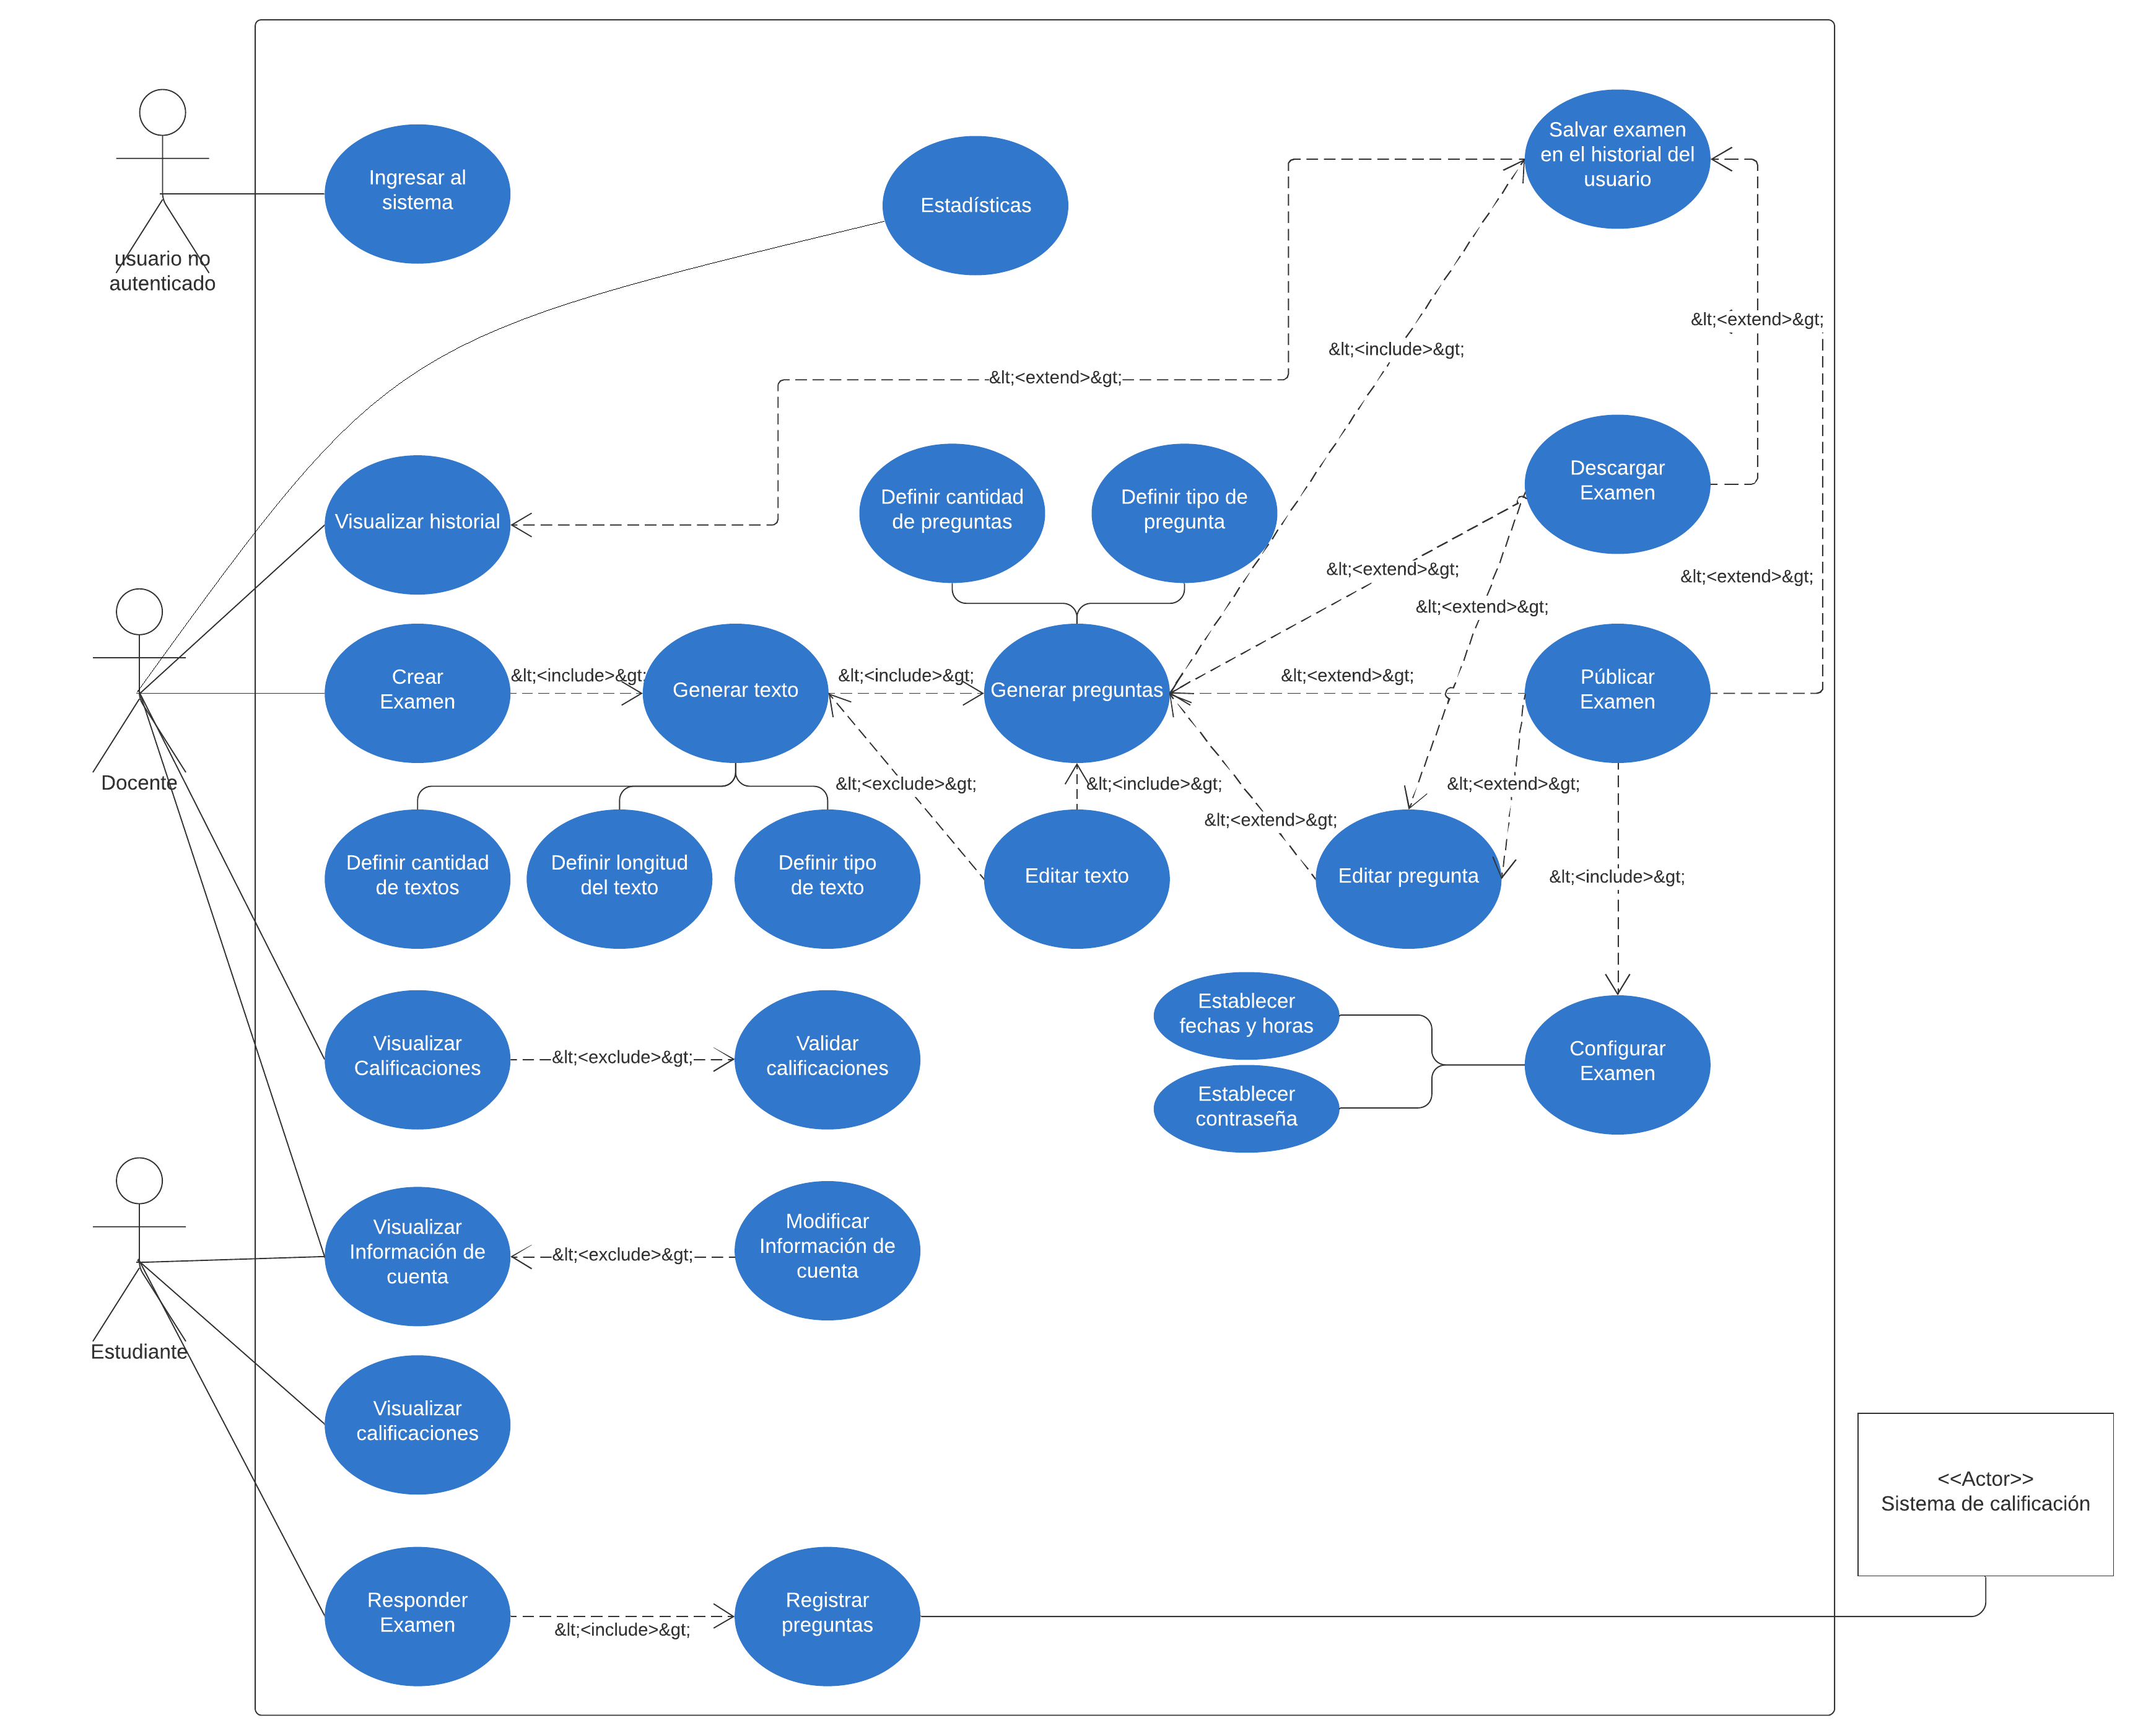
\includegraphics[width=6.4in,height=4.3in]{Images/Diagrama_casos_uso_GQuestions.png}
	    \caption{Diagrama de casos de uso - GQuestions}
	    Fuente: Elaboración propia
        \label{fig:section}
	\end{Center}
    \end{figure}

    \newpage
    \subsubsection{Modelo de base de datos}
    \begin{justify}
    Un modelo de base de datos es la estructura lógica que adopta la base de base datos, incluyendo las relaciones y limitaciones que determinan cómo se almacenan y organizan, y cómo se accede a los datos. Así mismo, un modelo de base de datos también define qué tipo de operaciones se pueden realizar con los datos, es decir, que también determina cómo se manipulan los mismos, proporcionando también la base sobre la que se diseña el lenguaje de consultas \cite{54}. %https://ayudaleyprotecciondatos.es/bases-de-datos/modelos/
    
    El modelo de base de datos del prototipo web se realizó bajo un modelo de base de datos relacional, en la figura 5.1.3 se presenta el modelo entidad-relación completo.
    \end{justify}
    
    \begin{figure}[H]
	\begin{Center}
		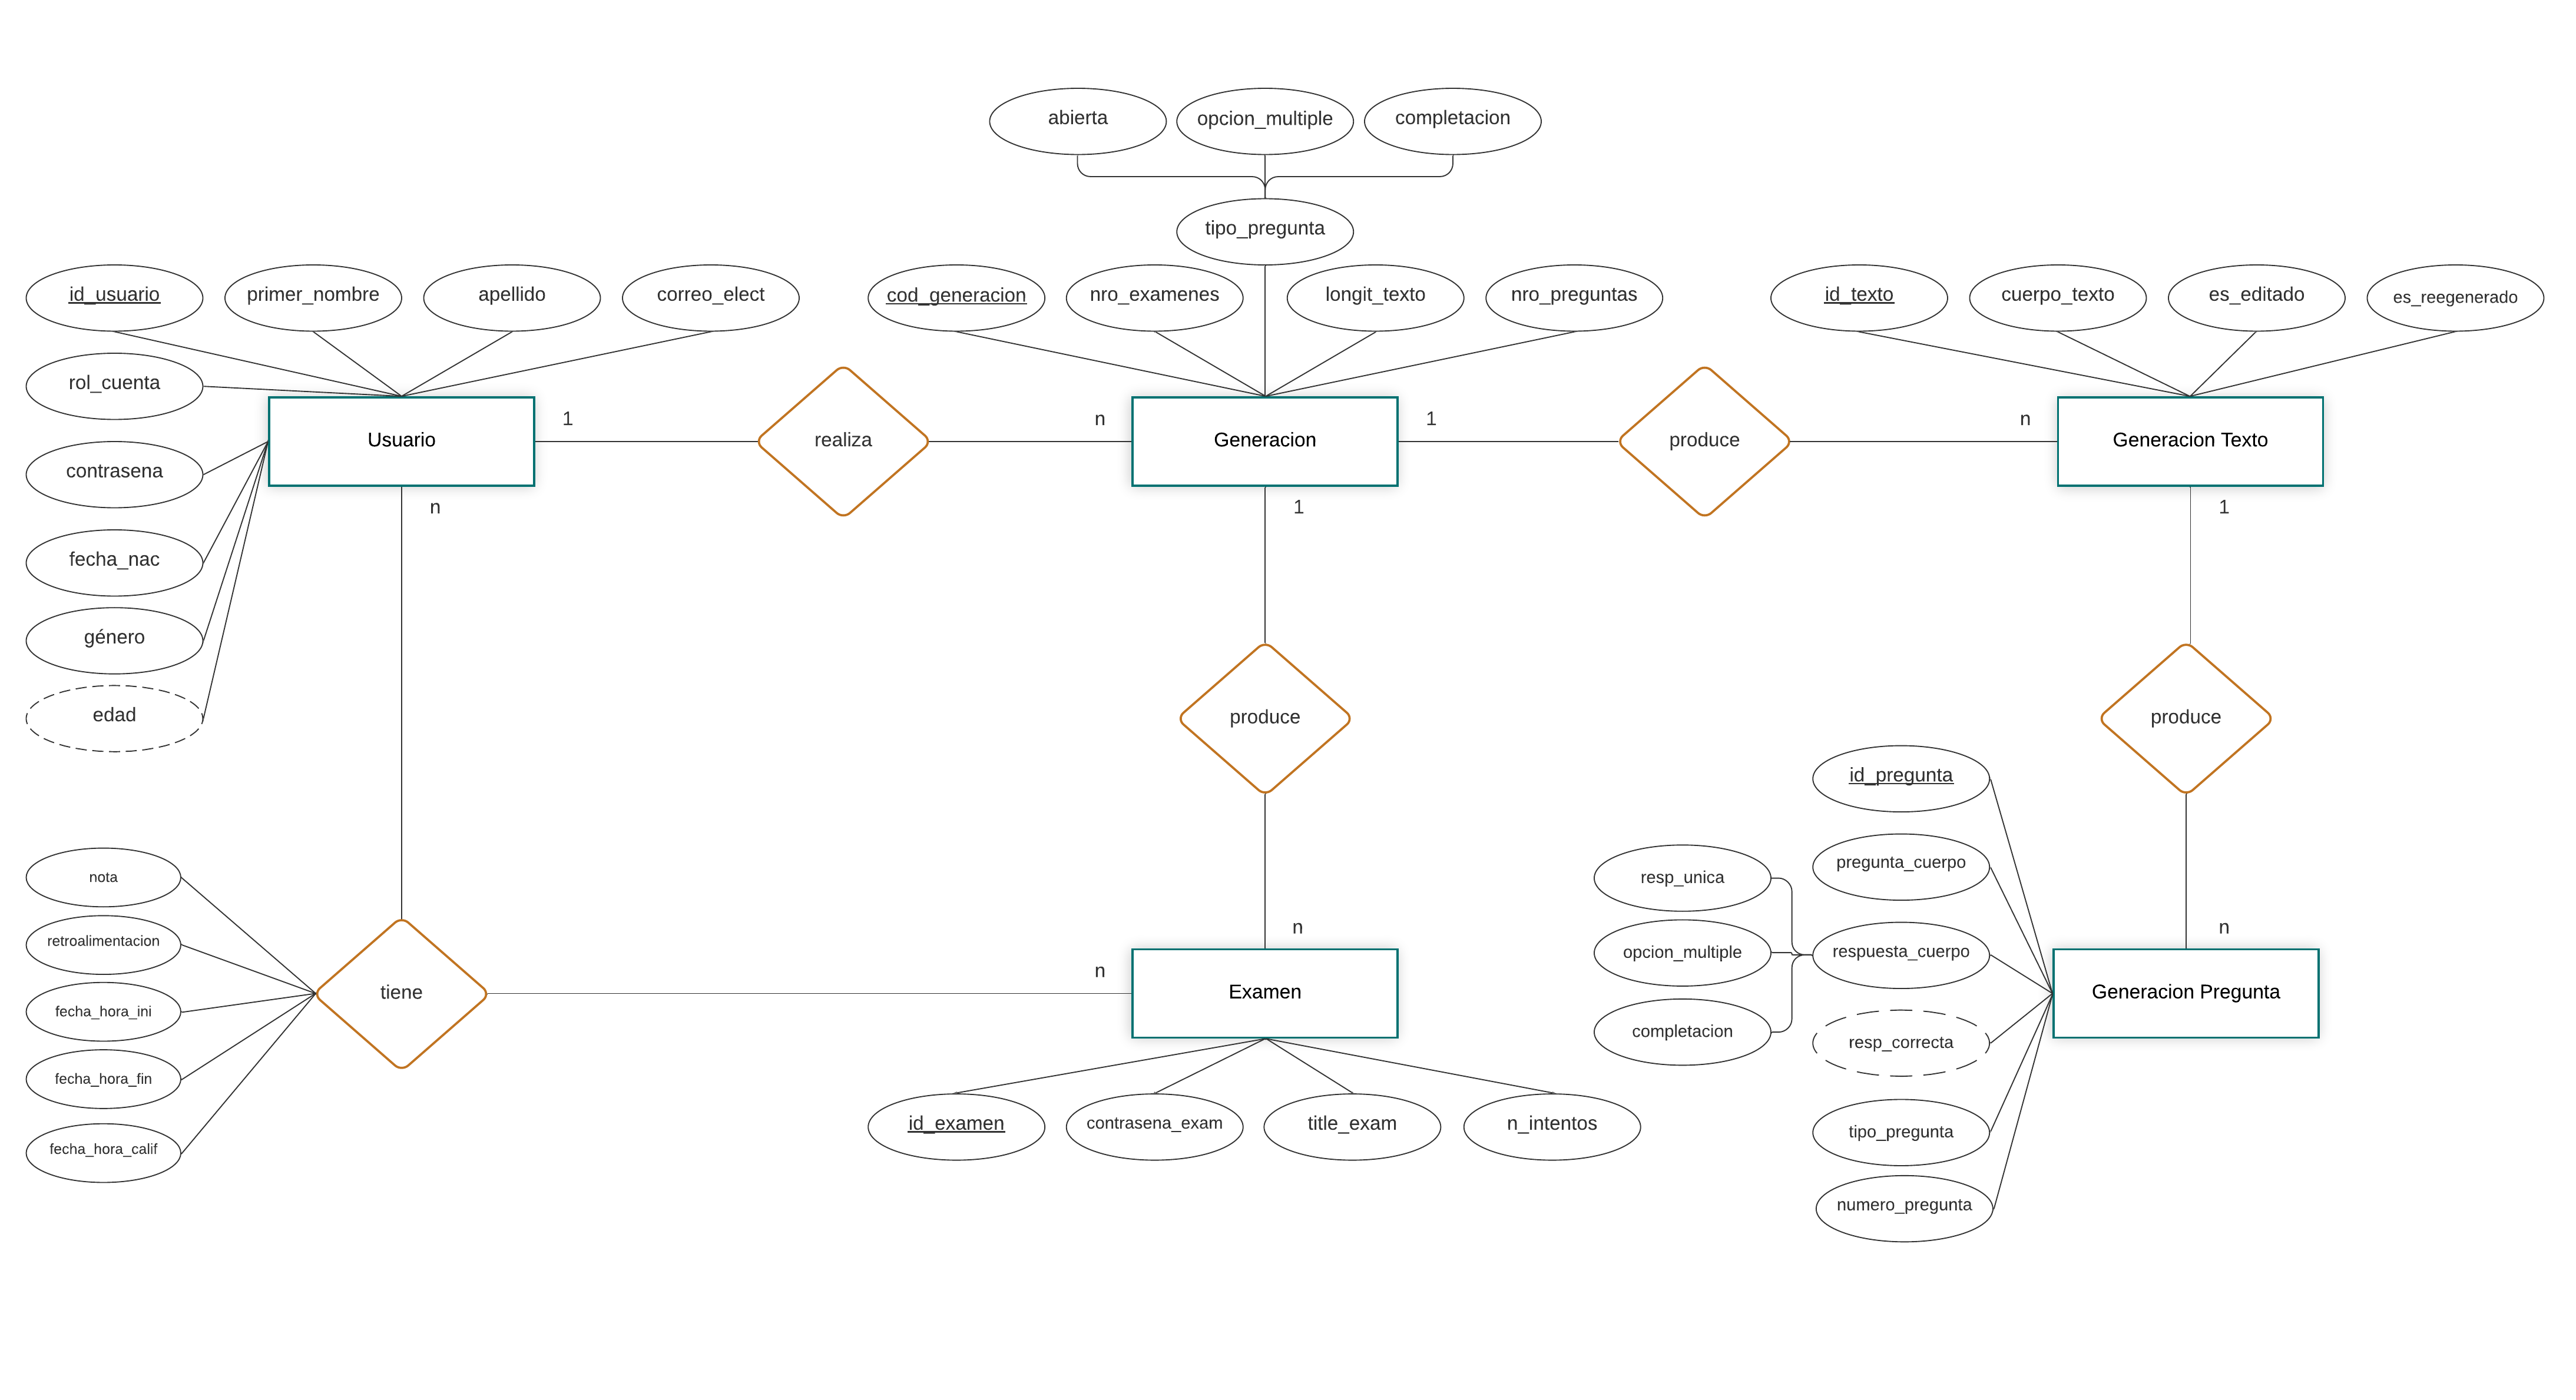
\includegraphics[width=6.4in,height=4.3in]{Images/Diagrama-ER-DBMS.png}
	    \caption{Modelo Entidad Relación - GQuestions}
	    Fuente: Elaboración propia
        \label{fig:section}
	\end{Center}
    \end{figure}
    
    \newpage
    \subsubsection{Diagrama de despliegue}
    
    \begin{justify}
    En el diagrama de despliegue se muestra la arquitectura de ejecución del prototipo web, en donde se incluyen nodos, entornos de ejecución tanto de software como de hardware y el middleware que los conecta. El fin de este diagrama es poder entender cómo se desplegará el sistema.
    \end{justify}
    
    \begin{figure}[H]
	\begin{Center}
		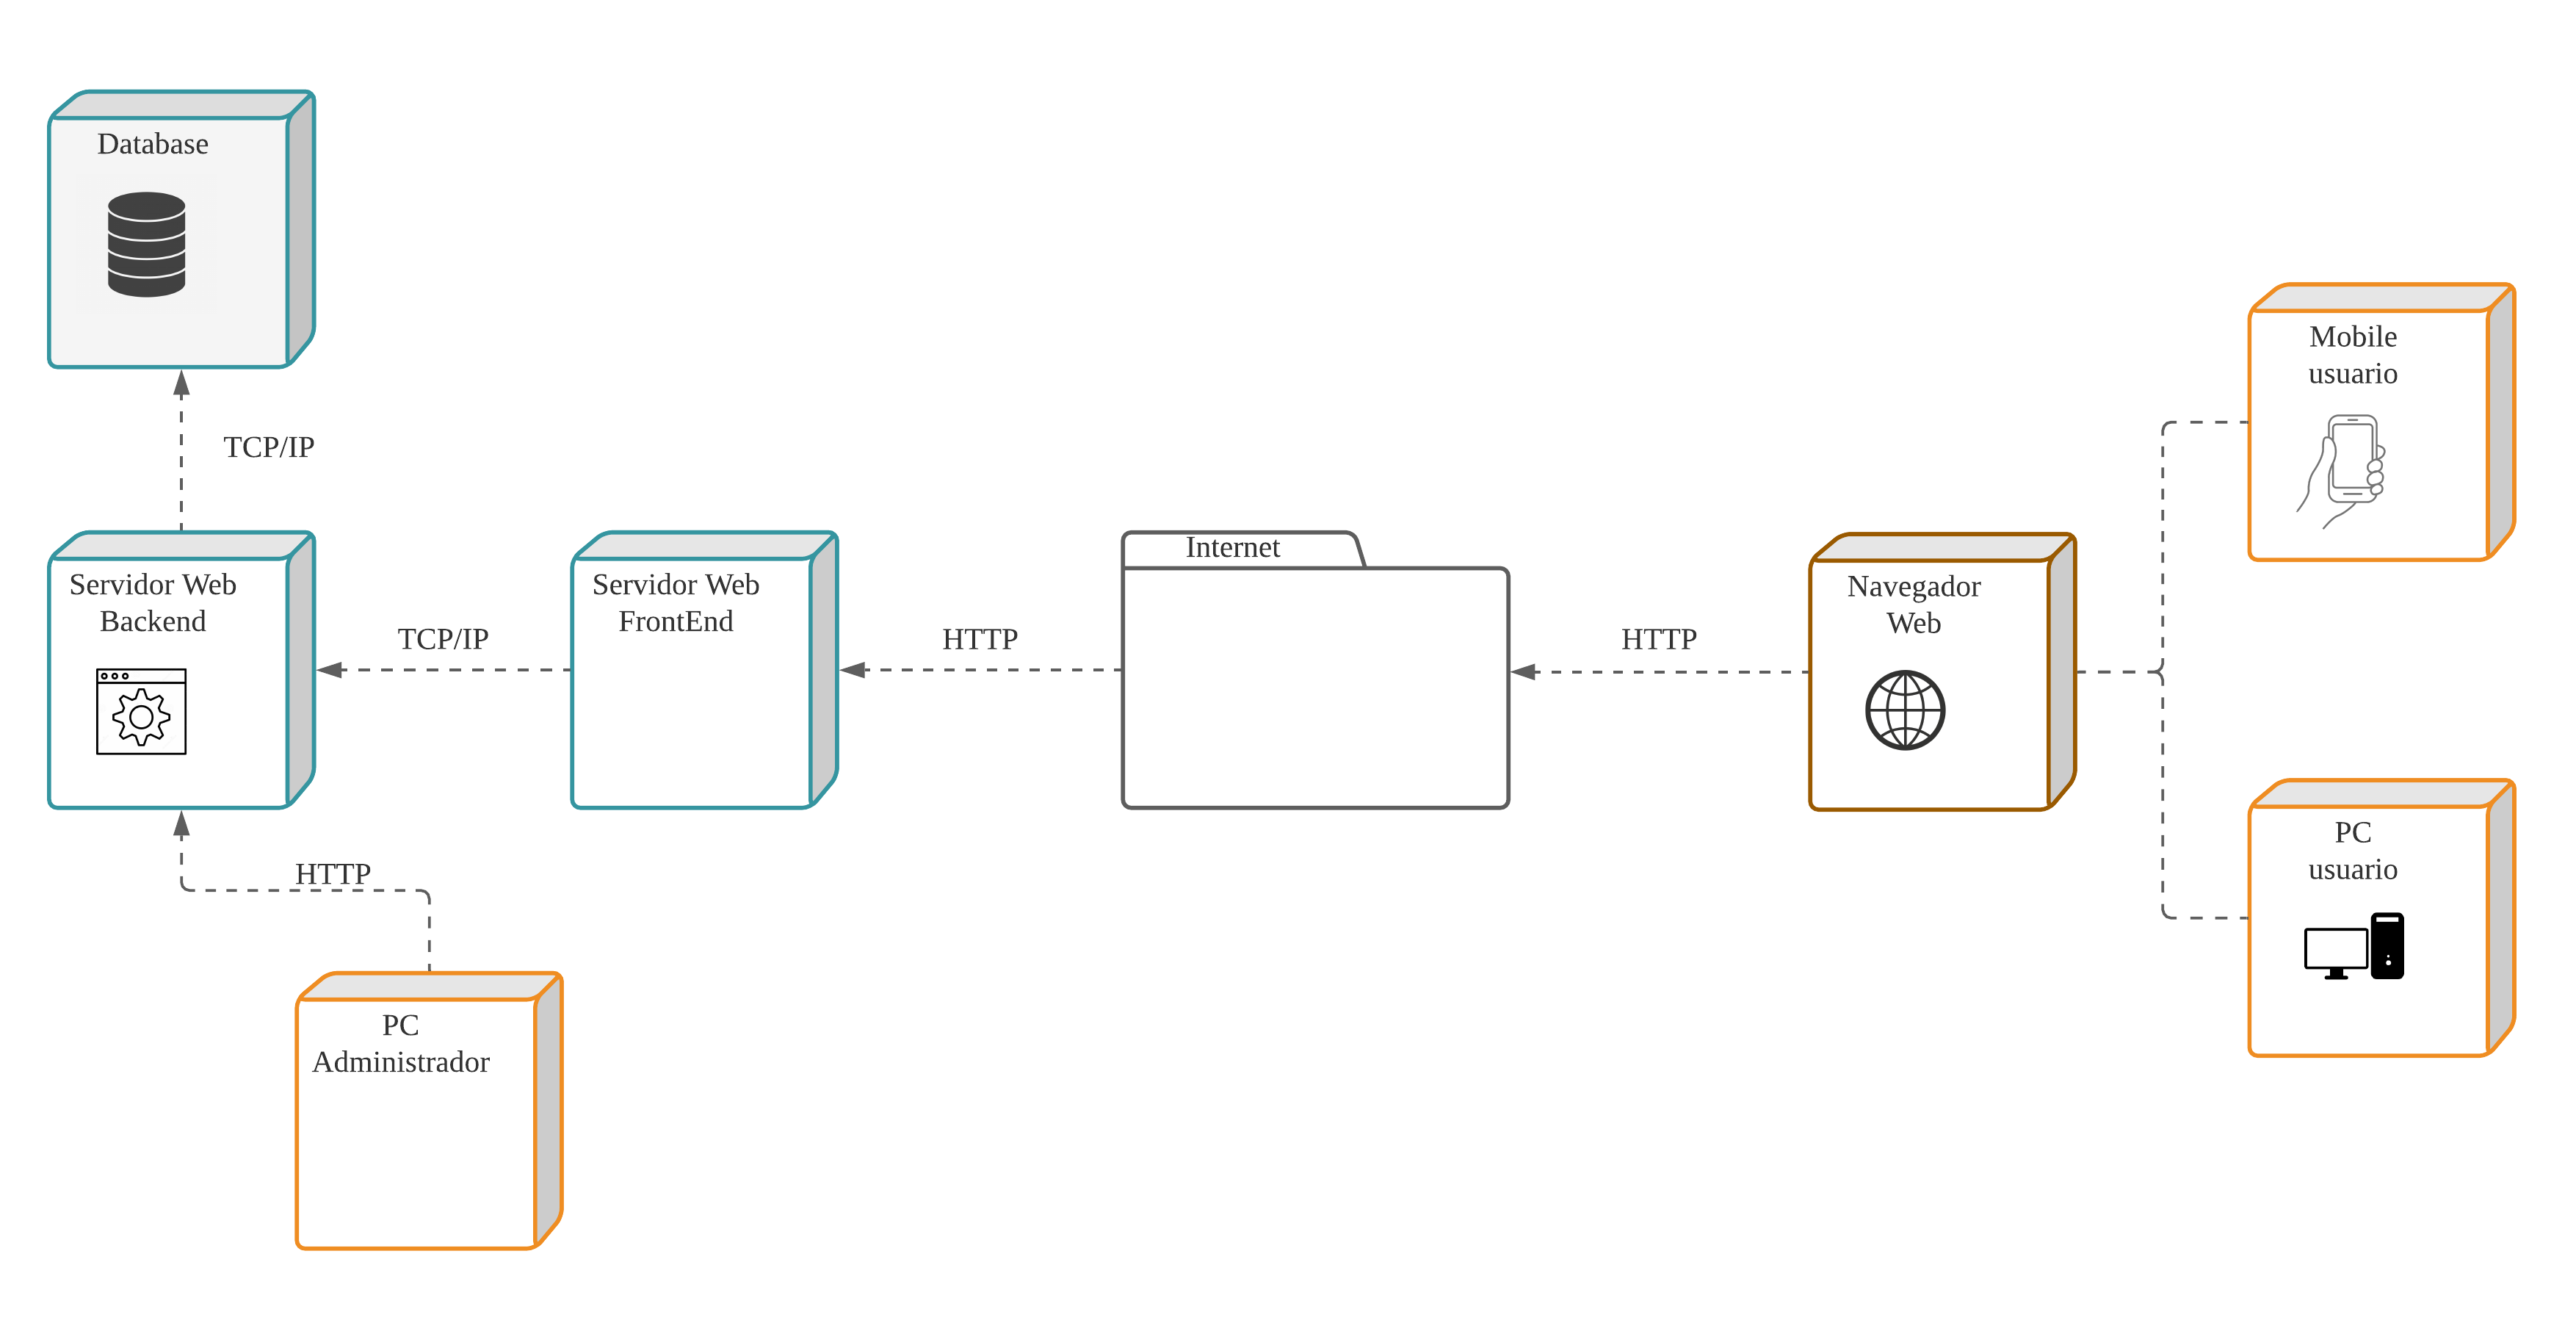
\includegraphics[width=6.4in,height=3.5in]{Images/diagrama_despliegue_GQuestions.png}
	    \caption{Diagrama de despliegue - GQuestions}
	    Fuente: Elaboración propia
        \label{fig:section}
	\end{Center}
    \end{figure}
\end{document}